\section{Durchführung}
Wie in der Darstellung \ref{fig:KA} zusehen besteht der Aufbau nicht nur aus
dem Michelson-Interferometer. Sondern auch aus einer Messzelle die evakuiert und
mit einem Gas gefüllt werden kann. Dahinter befindet sich einer der Spiegel des
Interferometers, welcher durch einen Motor den Spiegel verschiebt. Der Detektor
besteht aus einem Photoelemnt mit einem Verstärker und einem Zählwerk, welches
die Intesitätsmaxima zählt. \\
Zuerst muss das Interferometer so justiert werden, dass ein klares Interferenzmuster
vor dem Photoelement zu sehen ist. Dies wird unter Zuhilfenahme des justierbaren
Spiegels erreicht.\\
Zur Bestimmung der Wellenlänge des vom Laser ausgesendeten Lichts nun das Zählwerk
auf Null gestellt und die Messung startet wenn der Motor den Spiegel bewegt.
Nun wird abgewartet bis ca. 1000 Intensitätsmaxima gezählt wurden und
ließt den Verschub $\Delta d$ des Spiegels an der einer Messschraube ab.
Dies wird neun weitere Male wiederholt.\\
Zur Bestimmung des Brechungsindexes wird die Messzelle evakuiert und dann wieder
mit dem gewünschten Gas befüllt. Dabei werden wieder die Intensitätsmaxima
gezählt. Für jedes Gas wird dieser Vorgang wieder neun weitere Male wiederholt.

\label{sec:Durchführung}
\begin{figure}
  \centering
  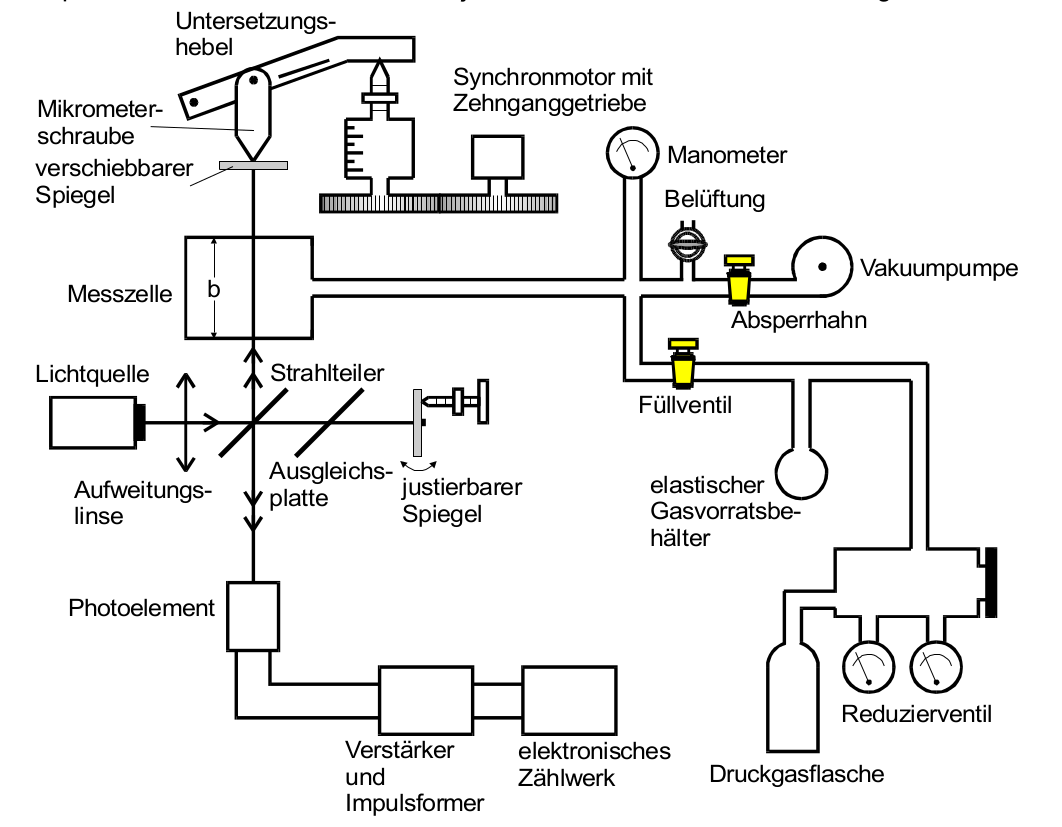
\includegraphics[height=5cm]{logos/Aufbau.png}
  \caption{Schematische Darstellung des kompletten Versuchsaufbaus \cite{Anleitung}. }
  \label{fig:KA}
\end{figure}
